\section{Normalizacijske i regularizacijske tehnike}
Prenaučenost je jedna od najvećih izazova pri treniranju modela strojnog učenja, a opisuje situaciju u kojoj pokušava naučiti ne samo važne trendove u podatcima, nego i šum koji neizbježno s njima dolazi. Osnovni načini kojima pokušavamo minimizirati vjerojatnost ovog problema jest korištenjem regularizacije i normalizacije. Regularizacija je bilo koja tehnika kojom, djelovanjem na parametre modela, težimo poboljšati sposobnost generalizacije, dok kod normalizacije utječemo na ulaze modela (kod neuronskih mreža, svakog sloja zasebno). S napretkom u istraživanju dubokih mreža, napredovale su i tehnike regularizacije i normalizacije. U ovom odjeljku, ukratko ćemo predstaviti metode koje se često koriste pri treniranju generativnih suparničkih modela.

\subsection{Regularizacija}
\subsubsection{$L_2$ regularizacija}
$L_2$ regularizacija oblik je regularizacije koji je vrlo raširen ne samo u treniranju dubokih mreža, nego i kod ostalih modela strojnog učenja. Osnovna pretpostavka jest da modeli koji postaju prenaučeni, postaju vrlo osjetljivi na male varijacije u ulaznim podatcima. Ovo se manifestira kao parametri koji imaju veliku normu te tako pojačavaju efekt šuma. Ideja je da na neki način ograničimo njihovu normu, što možemo postići malom modifikacijom funkcije gubitka modela. Pretpostavimo da model ima funkciju gubitka $L(\vec{x};\vec{\theta})$. Tada bi model s $L_2$ regularizacijom imao sljedeću funkciju kao funkciju gubitka:
\begin{equation*}
L^*(\vec{x};\vec{\theta}) = L(\vec{x};\vec{\theta}) + \frac{\lambda}{2}\|\vec{\theta}\|_2^2, 
\end{equation*}
gdje je $\|\vec{\theta}\|_2$ $L_2$ norma parametara modela. Ovime kažnjavamo model s prevelikim parametrima, a hiperparametar $\lambda$ određuje kompromis između minimizacije funkcije gubitka i norme parametara. 

Osim $L_2$ norme, u praksi se koriste i $L_1$ te $L_0$ da bi se ograničili parametri. Međutim, u kontekstu generativnih suparničkih mreža, najpovoljnija je upravo $L_2$ norma jer je svuda derivabilna, što nije istinito za ostale ovdje navedene norme.

\subsubsection{Spektralna normalizacija}
Spektralna normalizacija \citep{miyato2018spectral} zapravo je vrsta regularizacije jer utječe na težine modela, unatoč svome imenu, i karakteristično se koristi samo kod generativnih suparničkih modela. Ideja ove tehnike leži u činjenici da se povoljnim za stabilnost treniranja pokazala $K$-Lipschitzova neprekidnost diskriminatora \citep{qi2017losssensitive}. Prema definiciji, Lipschitzova norma vektorske funkcije $g(\vec{x})$ jest $\|g\|_{Lip} = \sup_{\vec{x}}\sigma(\nabla g(\vec{x}))$, gdje je $\sigma(A)$ spektralna norma matrice $A$, tj. 
\begin{equation}
\sigma(A) = \|A\|_2 = \sqrt{\lambda(A^T A)},
\end{equation}
a $\lambda$ je najveća svojstvena vrijednost matrice matrice $A^T A$. Za linearni sloj duboke mreže s matricom težina $W$, dobivamo $\|g\|_{Lip} = \sup_{\vec{x}}\sigma(\nabla g(\vec{x})) = \sup_{\vec{x}}\sigma(W) = \sigma(W)$. Koristeći činjenicu da je $\sigma(p \cdot W) = p \cdot \sigma(W)$, što je trivijalno za pokazati, vrijedi da je $\sigma(W / \sigma(W)) = 1$, odnosno promatrani linearni sloj zadovoljava 1-Lipschitzovu neprekidnost. Nadalje, iz svojstva $\|g_1 \circ g_2\|_{Lip} \leq \|g_1\|_{Lip} \cdot \|g_2\|_{Lip}$, slijedi i da je cijela mreža 1-Lipschitz neprekidna funkcija ako to svojstvo vrijedi za svaki sloj. Zato regulariziramo težine sloja $k$ kao $W_k \leftarrow  W_k / \sigma(W_k)$.
Međutim, u praksi je preskupo u svakom koraku optimizacije izračunavati svojstvene vrijednosti. Autori zato predlažu brzu metodu aproksimacije koju izlažu u svom radu, ali ona izlazi izvan opsega ovoga rada.

\subsubsection{Gradijentna kazna}
Gradijentna kazna \engl{Gradient penalty} \citep{gulrajani2017improved} također je tehnika kojim se pokušava osigurati Lipschitzova neprekidnost diskriminatora. Analizirajući učenje diskriminatora kad se koristi Wassersteinov gubitak uz ograničavanje težina na interval $[-c, c]$, autori su primijetili da 1) diskriminator nije sposoban modelirati složene funkcije te 2) ovisno o odabiru konstante $c$, učenje može rezultirati iščezavajućim ili eksplodirajućim gradijentima. Predložena alternativa temelji se na činjenici da optimalni diskriminator ima gradijent norme jednak 1, koju su autori dokazali u spomenutom radu. Zato predlažu sljedeću modifikaciju funkcije gubitka diskriminatora:
\begin{equation}
L^* = \mathbb{E}_{\vec{z} \sim p_{\vec{z}}}\left[D(G(\vec{z}))\right] - \mathbb{E}_{\vec{x} \sim p_{\mathcal{D}}} \left[D(\vec{x})\right] + \lambda \mathbb{E}_{\vec{\hat{x}} \sim p_{\vec{\hat{x}}}} \left[\left(\|\nabla_{\vec{\hat{x}}} D(\vec{\hat{x}})\|_2 - 1 \right) ^2 \right] 
\end{equation}
U odnosu na originalni optimizacijski problem, formulirali smo zadatak kao minimizaciju umjesto maksimizacije. Dodatni član u izrazu služi da bi se kaznio gradijent koji previše odstupa od optimalne vrijednosti, a $\lambda$ je hiperparametar kojim modeliramo jakost kazne (autori predlažu $\lambda = 10$). Osim toga, pokazuje se da je skupo kažnjavati gradijent svuda: autori predlažu odabir nasumične točke na spojnici uzoraka iz $p_{\mathcal{D}}$ i $p_{model}$ prema uniformnoj distribuciji te kažnjavanje gradijenta u toj točki. Na slici \ref{gp_calc} je prikazana implementacija odabira u programskom jeziku Python.

\begin{figure}[h]
\centering
		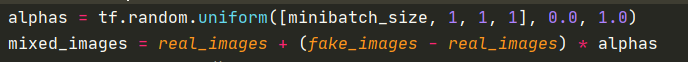
\includegraphics[width=0.8\textwidth]{images/gp_calc.png}
\caption{Implementacija odabira točaka sa spojnici uzoraka iz trenutnih minigrupa stvarnih i generiranih slika koristeći programski jezik Python i radni okvir Tensorflow}
\label{gp_calc}
\end{figure} 

Potrebno je napomenuti i da je ovaj oblik regularizacije vremenski nešto složeniji od prethodno navedenih, ali nije ograničen samo na Wassersteinov gubitak, nego se vrlo lako mogu ugraditi i druge funkcije gubitka.

\subsection{Normalizacija}
\subsubsection{Normalizacija nad grupom}
Normalizacija nad grupom \engl{Batch Normalization} \citep{ioffe2015batch} temelji se na opažanju da je treniranje mreža lakše ako su im na ulazu normalizirani podatci. Kako se mreža sastoji od više slojeva, cilj bi nam bio da svaki sloj primi normalizirani ulaz, uz razuman vremenski trošak. Budući da mrežu učimo na manjim grupama podataka, možemo procijeniti očekivanje $\vec{\mu}$ i varijancu $\sigma^2$ svake grupe te pomoću njih normalizirati grupu:
\begin{equation}
\hat{\vec{x}} = \frac{\vec{x} - \vec{\mu}}{\sqrt{\vec{\sigma}^2 + \epsilon}}
\end{equation}
Operacija korjenovanja, kvadriranje i dijeljenje u ovom se slučaju odvijaju po elementima, a $\epsilon$ jest mala konstanta dodana u izraz radi numeričke stabilnosti. Iako nam je potrebna minigrupa da bismo odredili očekivanje i varijancu, dimenzionalnost tih vektora ovisi o dimenzionalnosti vektora $\vec{x}$, a ne broju uzoraka u minigupi. Kako ipak tijekom normalizacije gubimo određenu sposobnost reprezentacije zbog gubitka srednje vrijednosti i odstupanja, nakon normalizacije afino transformiramo dobiveni vektor:
\begin{equation}
\label{affine}
\vec{h} = \vec{\alpha} \odot \vec{\hat{x}} + \vec{\beta}
\end{equation}
Ovdje $\odot$ označava Hadamardov produkt (produkt po elementima). $\vec{\alpha}$ i $\vec{\beta}$ tada također postaju parametri koje učimo gradijentnim spustom, ali nam omogućavaju lakšu manipulaciju distribucijom izlaza svakog sloja - uobičajeno je da se normalizacija nad grupom primjenjuje prije aktivacijske funkcije. 

Još jedno važno implementacijsko pitanje je kako koristiti normalizaciju nad grupom nakon što je model naučen. Naime, nakon što se učenje završi, više se podatci ne predaju modelu u minigrupama, nego mora biti omogućeno i obrada pojedinačnih ulaza. Zato se u fazi eksploatacije koriste druge vrijednosti za očekivanje i varijancu, dobivene temeljem očekivanja i varijanci svih minigrupa tijekom učenja:
\begin{equation}
\vec{\mu} = \mathbb{E}\left[\mu_k\right], \quad \vec{\sigma}^2 = \mathbb{E}\left[\vec{\sigma}^2_k\right]
\end{equation}

\subsubsection{Normalizacija sloja}
Normalizacija sloja \citep{ba2016layer} metoda je normalizacije razvijena zbog neprikladnosti normalizacije po grupama za mreže s povratnim vezama, a u kontekstu generativnih suparničke mreža prvi put je primijenjena nešto kasnije \citep{gulrajani2017improved} iz sličnog razloga. Naime, koristimo li normalizaciju po grupama, učimo diskriminator mapiranju između \textit{minigrupe ulaza u minigrupu izlaza}, što potencijalno uvodi korelaciju među primjerima. S druge strane, gradijentnom kaznom kažnjavamo gradijent diskriminatora za svaki primjer zasebno što zahtijeva metodu normalizacije koja ne uvodi korelaciju među ulazima. Ovdje na scenu stupa normalizacija po sloju. Ideja je da se očekivanje i varijanca odrede prema izlazima sloja za jedan primjer, umjesto prema minigrupi. Ako pretpostavimo da redovi matrice $H$ sadrže izlaze nekog sloja za danu minigrupu: u slučaju normalizacije po minigrupama, potrebne parametre procjenjujemo po redovima matrice $H$, a u slučaju normalizacije po sloju, po stupcima dane matrice. Tako izlaz za svaki primjer kod normalizacije sloja ima vlastito očekivanje i varijancu. Odredivši parametre, normaliziramo izlaz prema
\begin{equation}
\hat{\vec{x}} = \frac{\vec{x} - \vec{\mu}}{\sqrt{\vec{\sigma}^2 + \epsilon}}
\end{equation}
te primjenjujemo afinu transformaciju na dobiveni vektor (izraz \ref{affine}). Kao i ranije, učimo parametre afine transformacije.

Prednosti ovog pristupa su što ne postoji razlika u korištenju sloja tijekom faze eksploatacije u odnosu na fazu korištenja, primjenjiva je i kad veličina minigrupe nedovoljna za dobru aproksimaciju očekivanja i varijance, osigurava da su izlazi sloja za različite primjere međusobno neovisni, ali uvode korelaciju između izlaza za isti primjer.